\chapter{Methodology}  \label{ch:methodology}

\begin{table}[h]
\centering
 \begin{tabular}{l l} 
 \hline
 SYMBOL & DESCRIPTION \\ 
 \hline
 $K$ & Number of Topics \\  
 $V$ & Number of words in the vocabulary \\
 $M$ & Number of documents \\
 $N$ & Number of words in the document \\
 $N_{d=1..M}$ & Number of words in document d\\
 $\alpha$ & Collection of all $\alpha$ = $ \{ \alpha_{1},\alpha_{2}, ... , \alpha_{K}\}$ \\
 $\alpha_{k=1...K}$ & Hyperparameter for dirichlet prior distribution of topic $k$ \\
 $\beta$ &  Collection of all $\beta$ = $\{\beta{1},\beta{2}, ... , \beta_{K}\}$ \\
 $\beta_{w=1...V}$ & Hyperparameter for dirichlet prior distribution of a word $w$ in a topic \\
 $\varphi_{k=1...K}$ & Distribution of words in topic $k$ \\
 $\varphi_{k=1...K, w=1...V}$ & Weight of  word $w$ in topic $k$  \\
 $\theta{d=1...M}$ & Distribution of topics in document $d$  \\
 $\theta{d=1...M, k=1...K}$ & Weight of  topic $k$ in document $d$ \\
 $z_{d=1...M, w=1...N_d}$ & Assigned topic of word $w$ in document $d$\\
 $Z$ & Topic of all words in documents \\
 $w_{d=1...M, w=...N_d}$ & Assigned word w in document d \\ 
 $W$ & Words in all documents \\ 

 \hline
 \end{tabular}
\caption{Complete notation of LDA}
\label{tab:table1}
\end{table}

\section{Topic Modelling}\label{lda:tm}
Topic models are models used to find latent topics in mostly large unstructured collections of documents. Topic modelling assumes that documents are a mixture of topics, while topics are a distribution of words. \cite{Blei2010ProbabilisticModels}. Where humans have a hard time to find a structure, topic modelling uses statistical methods for analysing words for topic discovery. This makes it possible to compare topics with each other and to find similar documents without necessarily having any prior knowledge of your documents. The application of topic modelling is wide and is very powerful, making it a very popular for exploration of data. 

The machine learning and text mining area have focused a lot on probabilistic topic models in recent years. Models like probabilistic latent semantic analysis (PLSA) and sentiment analysis are used for applications ranging from document clustering, topic modelling and retrieval systems \cite{Lu2011InvestigatingLDA}. Optimising models is a challenging task, making usage of a high range from inference e.g. variational, stochastic and Markov chain Monte Carlo \cite{Hoffman2016MarkovModels}. The model that is used in this research and build upon the before mentioned models will be discussed in great length below.


\section{Latent dirichlet allocation}\label{lda:lda}
In natural language processing, \textit{Latent dirichlet allocation} (LDA) is an unsupervised machine learning technique introduced in 2003 for Topic modelling \cite{Blei2003LatentAllocation}. The notation used for LDA can be seen in Table \ref{tab:table1}. 

LDA makes use of a generative probabilistic model of a collection of documents \textbf{M} (corpus) to discover latent topics. Fig \ref{fig:LDA} represents the plate notation of LDA. For a more understandable model consider Fig \ref{fig:LDA_example}. The model assumes that each document \textbf{N} in the corpus consists of a mixture of latent topics. These topics are a mixture of words \textbf{W} assigned to a topic from a fixed vocabulary \textbf{V}. \textbf{Z} notates the assignment of specific words to topics. The distribution of words $\theta$ for each topic is dependent on the sensitivity of $\alpha$. The probability distribution of topics in documents $\varphi$ are depended on the sensitivity of $\beta$. The number of topics \textbf{K} are predefined by the user. 

\begin{figure}
    \centering
    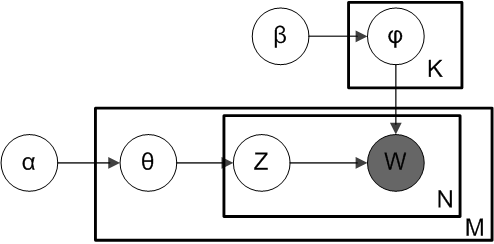
\includegraphics[width=10cm, height=5cm]{methodology/Smoothed_LDA.png}
    \caption{The smoothed LDA plate notation}
    \label{fig:LDA}
\end{figure}

The LDA model is defined in 3 steps and shown in Fig \ref{fig:LDA_example}:
\begin{enumerate}
    \item For each document, pick a topic from its assigned distribution over topics.
    \item Sample a word from the distribution over the words associated with the chosen topic. 
    \item  The process is repeated for all the words in the document.
\end{enumerate}

For a better understanding, look at the before mentioned Fig \ref{fig:LDA_example}. The topics are shown on the left side with their probability of words. On the right side, the document has a topic proportion. Every word gets assigned to a topic so that the topic proportion matches.  
In the original LDA model, assignments of words get updated every iteration through the corpus M. Restarting the process again until the LDA model converges and the topic and assignment are stale. The eventual quality of the model depends on the assumed hyperparameters $\alpha$ and $\beta$ and parameters $\theta$ and $\varphi$. For a better understanding of the parameters take a look at section \ref{lda:alphabeta} and section \ref{lda:thetavarphi}.

\begin{figure}
    \centering
    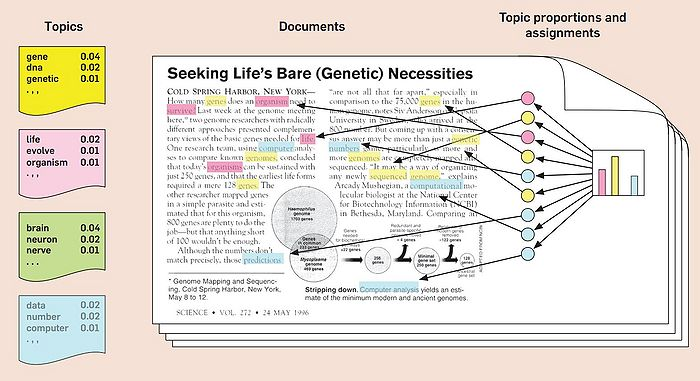
\includegraphics[scale=0.6]{methodology/700px-Illustrating_LDA.jpg}
    \caption{LDA applied to a document}
    \label{fig:LDA_example}
\end{figure}

\subsection{$\alpha$ and $\beta$ hyperparameters}  \label{lda:alphabeta}
The dirichlet is defined as the distribution over a distribution. Dirichlet is used to infer a posterior distribution after observations using a prior distribution \cite{Sethuraman2001APRIORS}. Hyperparameters are defined as parameters that assume a prior distribution before any evidence or information is taken into account. This distinguishes $\alpha$ and $\beta$ from the remaining parameters. $\alpha$ and $\beta$ are both dirichlet distributions. The hyperparameter value $\alpha$ is the parameter of the dirichlet prior on the per-document topic distributions. The result of a high value of $\alpha$ is a document with a mixture of most topics, while the low value leads to documents with more distinct topics. The $\alpha$ results in a corpus with distinct documents or more general documents topic assignments. The value $\beta$ is the parameter of the dirichlet prior of a word in a topic. A high value for $\beta$ means that the topics consists of distinct words, the low value of $\beta$ assumes topics are more generative. The $\beta$ will influence the general distribution of words in topics in the output of topics.

\subsection{$\theta$, $\varphi$ parameters}\label{lda:thetavarphi}
The parameters $\theta, \varphi$ are depend on the prior distributions $\alpha$ and $\beta$. $\theta$ is the document-topic distribution. $\theta$ is the weight of a topic in a document and because $\alpha$ is a prior distribution, $\theta$ assumes a distribution based on the previous assigned distribution. 
In the same way $\varphi$ is the weight of words in a topic. $\varphi$ in this case is dependent on the $\beta$.

\section{Online Latent dirichlet allocation} \label{lda:onlinelda}
The online variant of LDA was introduced  by Hoffman et al. in 2010.\cite{Hoffman2010OnlineAllocation} This new variation dealt with the problem earlier LDA models struggled with. The problem that LDA had was the computing of huge collections of documents. The online LDA can be used for massive and streaming documents without losing performance compared to the original LDA model, because it analyses the documents in batches instead of single observations with stochastic (random) optimisation.\cite{Beaver2012StochasticInference} 
